\chapter{Inleiding}
\label{inleiding}
%%%%%%%%%%%%%%%%%%%%%%%%%%%%%%%%%%%%%%%%%%%%%%%%%%%%%
%          Waarom configuratiemanagement?           %
%%%%%%%%%%%%%%%%%%%%%%%%%%%%%%%%%%%%%%%%%%%%%%%%%%%%%
Configuratiebeheergereedschappen zijn ontwikkeld om het leven van systeembeheerders makkelijker te maken.
De serverinfrastructuren die ze moeten onderhouden worden steeds uitgebreider en complexer.
Manueel elke server configureren kost niet alleen te veel tijd maar is ook erg foutgevoelig.
Er bestaan reeds verschillende oplossingen voor dit probleem.
Een eerste manier is scripts gebruiken.
Dit is al een stap in de goede richting maar is nog steeds niet voldoende: 
als de uitvoering van een script afgebroken wordt blijft het systeem in een onstabiele toestand.\cite{sysadvent}

Een andere manier om een verzameling gelijkaardige machines van hun initi\"ele configuratie te voorzien is het gebruik van images.
Daarbij wordt eerst \'e\'en machine manueel geconfigureerd en daarna wordt de volledige set-up gekloond naar de rest van de servers.
Deze methode werkt niet meer voor het verdere onderhoud van de configuraties.

%%%%%%%%%%%%%%%%%%%%%%%%%%%%%%%%%%%%%%%%%%%%%%%%%%%%%
%          Overgaan naar de cloud                   %
%%%%%%%%%%%%%%%%%%%%%%%%%%%%%%%%%%%%%%%%%%%%%%%%%%%%
Dit onderhoudsprobleem komt nog prominenter voor als de infrastructuur niet lokaal maar in de cloud gehost wordt.
Een groot voordeel van werken in de cloud is de flexibiliteit waarmee servers kunnen toegevoegd en weggenomen worden.
Dit proces gebeurt vaak zelfs automatisch waardoor manuele configuratie helemaal geen optie meer is. \todo{source?}
In een dergelijke omgeving is een tool die uit zichzelf de volledige infrastructuur kan beheren bijna een noodzaak.

%%%%%%%%%%%%%%%%%%%%%%%%%%%%%%%%%%%%%%%%%%%%%%%%%%%%%
%          Werking huidige tools                    %
%%%%%%%%%%%%%%%%%%%%%%%%%%%%%%%%%%%%%%%%%%%%%%%%%%%%%
Configuratiebeheergereedschappen (of CMS: Configuration Management Software, vanaf nu zal deze term gebruikt worden) zoals IMP\cite{IMP}, Puppet\cite{puppet}, CFEngine\cite{cfengine},\ldots laten toe op een effici\"ente manier IT-infrastructuren op te zetten en te onderhouden.
De gebruiker van een dergelijke tool specifi\"eert eerst een model dat de gewenste toestand van de volledige infrastructuur beschrijft.
Dit model bestaat uit een oplijsting van machines met de gewenste aanwezige resources (bestanden, mappen, services,\ldots) die ze moeten aanbieden.
Sommige tools laten ook toe samenhorende resources te groeperen in een concept, zoals een webserver of een databaseserver.
Dit vermijdt duplicatie van code in het model.

Bij het uitrollen van een model (een "deployment run") inspecteert de CMS de huidige toestand van elke machine en vergelijkt ze met de gewenste toestand.
Als er een verschil is maakt de CMS de nodige aanpassingen, indien niet onderneemt ze geen actie.
De beheerder van de verzameling systemen moet dus na het opstellen van de initi\"ele configuratie zelf geen stappen meer ondernemen om te verzekeren dat de gewenste situatie bereikt wordt.
Als er later nog aanpassingen moeten gebeuren moet enkel het model aangepast worden en een nieuwe deployment run gestart worden.

%%%%%%%%%%%%%%%%%%%%%%%%%%%%%%%%%%%%%%%%%%%%%%%%%%%%%
%          Dependencies gebruiken gaat beter        %
%%%%%%%%%%%%%%%%%%%%%%%%%%%%%%%%%%%%%%%%%%%%%%%%%%%%%
Een belangrijk aspect van elk gedistribueerd systeem zijn de afhankelijkheden die bestaan tussen de verschillende onderdelen.
Stel het voorbeeld van een LAMP-stack: een Linuxdistributie met de Apache webserver, de MySQL database en PHP.
Daar kan de webserver niet zijn volledige functionaliteit aanbieden voordat de database online is.
De webserver is dus afhankelijk van de databaseserver.
Zolang PHP niet ge\"installeerd is kan de webserver ook geen dynamische pagina's aanbieden.
Ze is dus ook afhankelijk van de PHP-installatie.
Een volledige mapping van de verschillende afhankelijkheden binnen de LAMP-stack is te zien op figuur \ref{fig:lamp_dep}.
\begin{figure}
    \begin{center}
    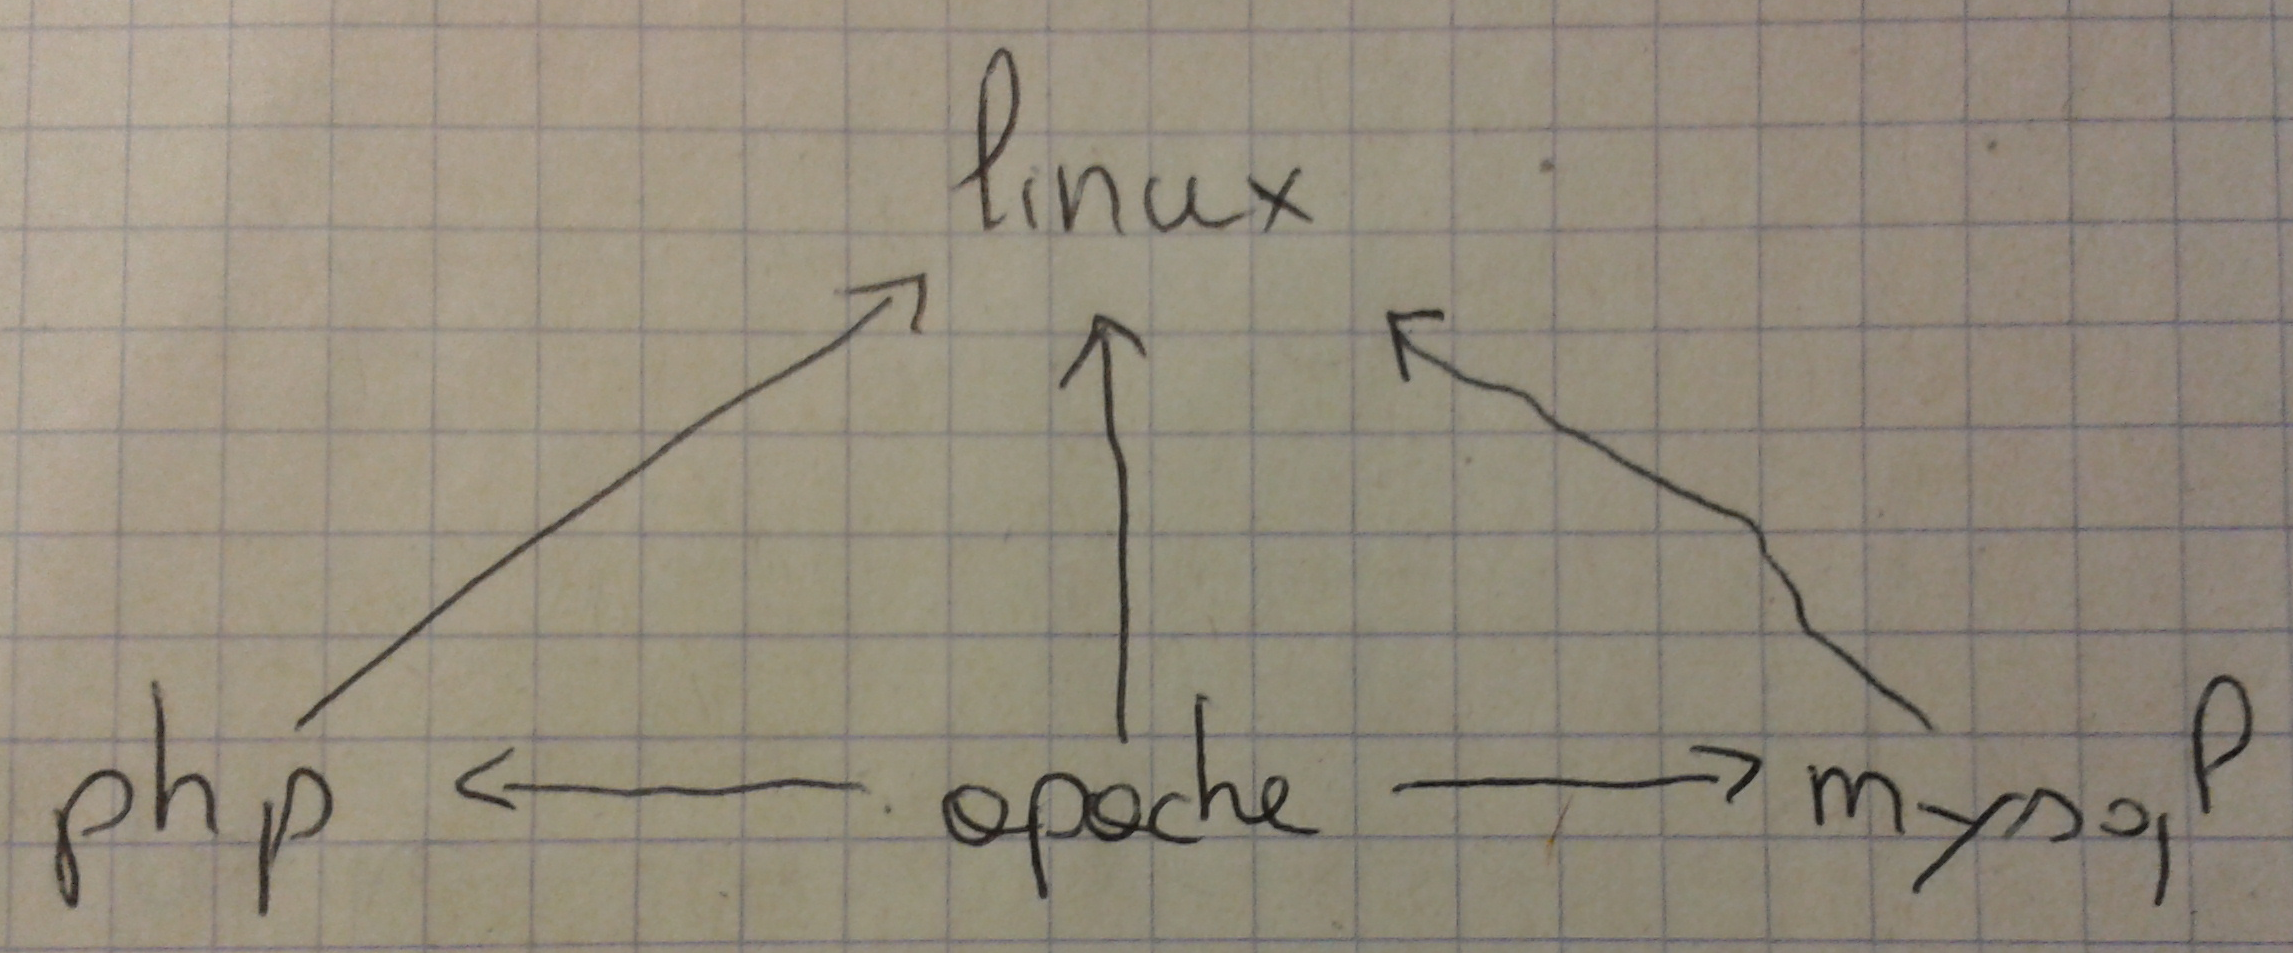
\includegraphics[width=0.6\textwidth]{images/lamp_dep.png}
    \caption{Grafische voorstelling van de afhankelijkheden binnen een LAMP-stack}
    \label{fig:lamp_dep}
    \end{center}
\end{figure}

Als deze afhankelijkheden niet gespecificeerd worden in het model kan de CMS er ook geen rekening mee houden.
Het kan dat de tool het model in een foute volgorde uitrolt: eerst de webserver, dan PHP en uiteindelijk de database.
De webserver zal bij het opstarten proberen te verbinden met de database, maar deze is nog niet online.
In de tijd tussen het opstarten van de webserver en de installatie van PHP zal ze ook geen dynamische webpagina's kunnen tonen.
Een op het eerste zicht succesvolle deployment run kan dus leiden tot een configuratie die niet volledig werkt.

In vergelijking met de beginsituatie is de toestand van de configuratie na de ene run wel al minder afwijkend van de gewenste situatie:
de verschillende pakketten, services en configuratiebestanden zijn al aanwezig.
Tijdens de volgende deployment run zal de Apache service herstart worden en dan zal ze wel kunnen connecteren met de database.

CMS zal nooit aanpassingen maken die zorgen voor een configuratie die verder afwijkt van het model dan voorheen.
Na een paar iteraties zal uiteindelijk altijd de gewenste configuratie bereikt worden. 
Grafisch wordt dit voorgesteld op figuur \ref{fig:convergentie}.
Het aantal iteraties is afhankelijk van de hoeveelheid afhankelijkheden die bestaan maar niet aanwezig zijn in het model.

\begin{figure}
    \begin{center}
    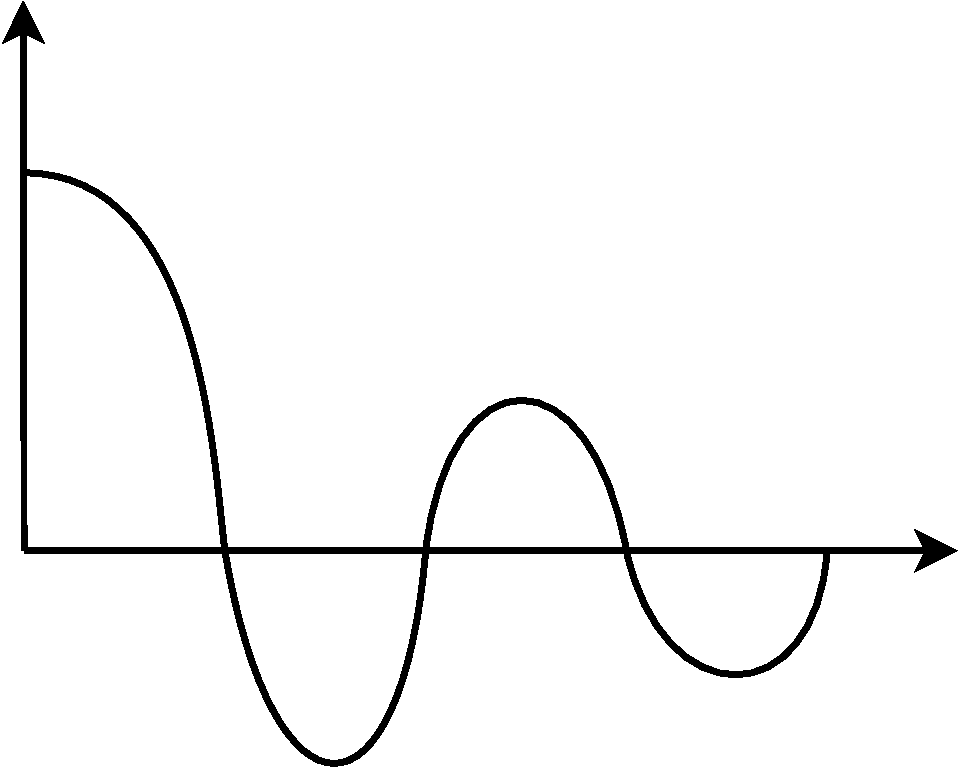
\includegraphics[width=0.6\textwidth]{images/convergentie.png}
    \caption{Grafische voorstelling van de convergentie na een reeks deployment runs.}
    \label{fig:convergentie}
    \end{center}
\end{figure}

\todo{``sprong'' in onderwerp}
Databases en webservers zijn abstracties die bestaan uit een verzameling basisobjecten zoals bestanden, pakketten en services.\todo{Beter woord voor abstracties}
Tussen deze objecten bestaan er natuurlijk ook afhankelijkheden, bijvoorbeeld tussen een bestand en de map waarin het staat:
als de CMS eerst probeert het bestand te cree\"eren en dan pas de map zal de deployment run slechts gedeeltelijk slagen want een bestand kan niet bestaan
zonder een bovenliggende map.
Figuur \ref{fig:file_dir_dep} stelt deze afhankelijkheid nog eens grafisch voor.
\begin{figure}
    \begin{center}
    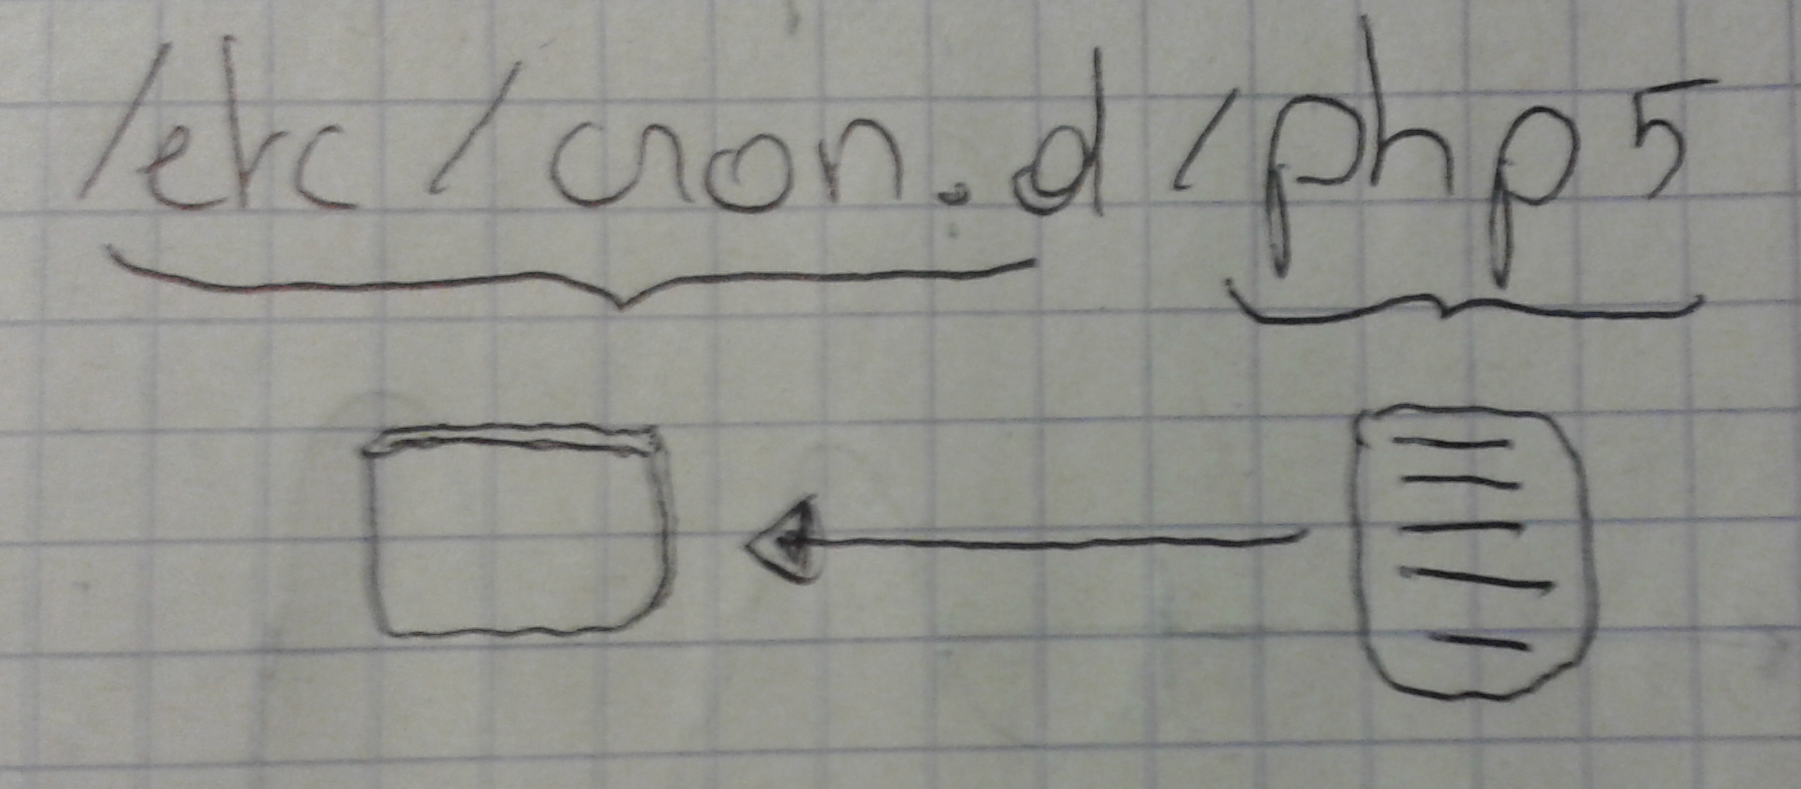
\includegraphics[width=0.6\textwidth]{images/file_dir_dep.png}
    \caption{Grafische voorstelling van de afhankelijkheid tussen een bestand en zijn parent folder}
    \label{fig:file_dir_dep}
    \end{center}
\end{figure}
In tegenstelling met het voorbeeld van de LAMP-stack zal de gebruiker direct na het uitrollen al zien dat er iets foutgaat.
De CMS zal namelijk tonen dat sommige resources niet werden uitgerold.
Bij de LAMP-stack werd alles succesvol uitgerold, maar de gebruiker kan pas zien dat er iets fout is als hij de logs van de Apache service bekijkt, of probeert een site te bezoeken.

We maken dus het onderscheid tussen twee gevallen: vereisten en afhankelijkheden.
In het geval van het bestand en de map is er sprake van een \textit{vereiste} die niet voldaan is: de map moet bestaan v\'o\'or het aanmaken van het bestand of deze wordt niet aangemaakt.
In het geval van de LAMP-stack houdt de CMS geen rekening met de \textit{afhankelijkheid} tussen de webserver en de databaseserver.
Alle resources worden foutloos aangemaakt maar toch werkt de uiteindelijke configuratie niet omdat een foute volgorde werd gehanteerd.
In beide gevallen is een extra deployment run nodig voordat de configuratie correct werkt.

Als de CMS wel rekening houdt met de afhankelijkheden en vereisten moet het model maar \'e\'en keer uitgerold worden.
Het doel van deze thesis is dan ook om uit te zoeken hoe de software deze extra informatie automatisch uit het model kan afleiden.\todo{Doel pas later vermelden?}

%%%%%%%%%%%%%%%%%%%%%%%%%%%%%%%%%%%%%%%%%%%%%%%%%%%%%
%          Afhankelijkheden met huidige tools       %
%%%%%%%%%%%%%%%%%%%%%%%%%%%%%%%%%%%%%%%%%%%%%%%%%%%%%
De huidige CMS laten toe om op het niveau van bestanden, packages en services vereisten en afhankelijkheden te specificeren.
De specificatie van een vereiste en een afhankelijkheid overlapt bij deze tools en wordt een ``requirement'' genoemd.
Bij het uitrollen van een model gebruikt de software die informatie om een volgorde op te leggen waarmee de verschillende objecten aangemaakt worden.

Deze tools compileren tijdens de deployment voor elke machine hun deel van het model.
Elke machine krijgt dus enkel informatie over wat hij zelf moet doen.
Afhankelijkheden en vereisten binnen eenzelfde machine verwerken is geen probleem maar tussen verschillende machines is dit niet mogelijk.
Als de LAMP-stack op \'e\'en machine ge\"installeerd wordt kan de gebruiker nog aangeven dat de Apache service afhankelijk is van de databaseservice en PHP.
Als daarintegen de Apache service op een machine draait en de MySQL-service op een andere kan de gebruiker dit niet meer aangeven.
De enige optie is dan meerdere keren het model uitrollen tot de configuratie correct werkt.
\footnote{Voor Puppet bestaat er wel een workaround, zie \cite{puppet-orchestration}. ``Orchestration'' CMS zoals Ansible kan dit wel. \big{TODO:} Verschil opzoeken en uitleggen hier of in related works?}

%%%%%%%%%%%%%%%%%%%%%%%%%%%%%%%%%%%%%%%%%%%%%%%%%%%%%
%     Afhankelijkheden en vereisten met IMP         %
%%%%%%%%%%%%%%%%%%%%%%%%%%%%%%%%%%%%%%%%%%%%%%%%%%%%%
IMP (Infrastructure Management Platform) is een nieuwe tool die momenteel nog in ontwikkeling is.
Ze verschilt op twee vlakken van de andere CMS: gebruik van het model tijdens het uitrolproces en de specificatie van vereisten en afhankelijkheden.%het/het

De andere aanpak tijdens het uitrollen van een model laat toe afhankelijkheden tussen hoog-niveau objecten te specificeren:
in tegenstelling tot de vorige tools krijgt elke machine het volledige model ter beschikking en niet alleen zijn eigen deel.
Machines kunnen zo niet alleen rekening te houden met afhankelijkheden en vereisten tussen eigen concepten maar ook tussen andere machines.

Vervolgens maakt IMP, in tegenstelling tot andere tools, wel het onderscheid tussen vereisten en afhankelijkheden:
een vereiste is net zoals bij de andere tools een requirement, maar afhankelijkheden worden gemodelleerd door middel van relaties tussen concepten.
\todo{Klopt dit volledig? Mijn heuristiek leidt afhankelijkheden af uit de relaties, maar dat is daarom niet het enige nut ervan.}
%IMP laat toe relaties te specifi\"eren tussen concepten, gelijkaardig aan de relaties tussen tabellen in een database.
%Uit deze relaties kunnen afhankelijkheden afgeleid worden.
Aangezien IMP tijdens het uitrollen elke machine het volledig model ter beschikking stelt kunnen intermachinale afhankelijkheden ook verwerkt worden.
%Aangezien deze relaties gespecifi\"eerd zijn tussen concepten, en concepten op verschillende machines uitgerold kunnen worden, kan IMP afhankelijkheden over verschillende machines verwerken.
%\todo{actief -> passief -> actief}

%%%%%%%%%%%%%%%%%%%%%%%%%%%%%%%%%%%%%%%%%%%%%%%%%%%%%
%          Probleem/doelstelling                    %
%%%%%%%%%%%%%%%%%%%%%%%%%%%%%%%%%%%%%%%%%%%%%%%%%%%%%
IMP kan het volledig model in \'e\'en keer uitrollen als het genoeg informatie krijgt in de vorm van vereisten en afhankelijkheden.
De doelstelling van deze thesis is aan de hand van heuristieken extra informatie uit het model halen en zo het aantal nodige deployment runs te verminderen.
De veronderstelling is wel dat degene die het model opstelt genoeg domeinspecifieke informatie aanlevert die door deze heuristieken gebruikt kan worden.

%%%%%%%%%%%%%%%%%%%%%%%%%%%%%%%%%%%%%%%%%%%%%%%%%%%%%
%          Kort: hoe oplossing + resultaten         %
%%%%%%%%%%%%%%%%%%%%%%%%%%%%%%%%%%%%%%%%%%%%%%%%%%%%%
\todo{Gebruik van ``dus''}
\big{TODO:} hoe oplossing + resultaten
